\documentclass[tikz,border=3.14mm]{standalone}
\usepackage{pgfplots}
\usetikzlibrary{decorations, arrows, arrows.meta}

\begin{document}
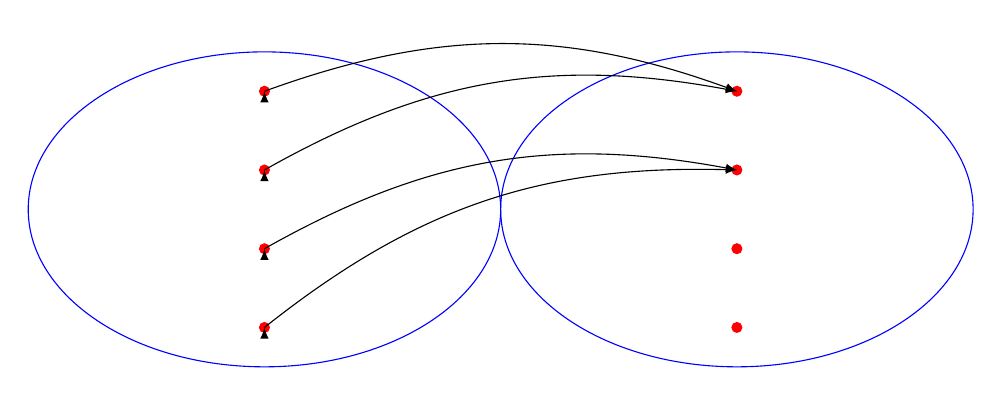
\begin{tikzpicture}

% Draw ovals
\draw[blue] (0,0) ellipse (3cm and 2cm);
\draw[blue] (6,0) ellipse (3cm and 2cm);

% Draw points in the first oval
\foreach \i/\y in {1/1.5, 2/0.5, 3/-0.5, 4/-1.5} {
    \fill[red] (0, \y) circle (2pt) coordinate (a\i);
}

% Draw points in the second oval
\foreach \i/\y in {1/1.5, 2/0.5, 3/-0.5, 4/-1.5} {
    \fill[red] (6, \y) circle (2pt) coordinate (b\i);
}

% Draw arrows to represent the mapping and its inverse
\foreach \i in {1,2} {
    \draw[-latex] (a\i) edge [bend left = 20] (6, 1.5);
}
\foreach \i in {3,4} {
    \draw[-latex] (a\i) edge [bend left = 20] (6, 0.5);
}

\end{tikzpicture}
\end{document}
